\subsection{Modelado de Contexto}
\label{subsec:Prop_Modelado}

Como se indica en la sección \ref{sec:MT_SensibilidadContexto} las ontologías son la estrategia de modelado de contexto que hemos seleccionado en este trabajo, la decisión se respalda en \textbf{\textit{(i)}}el estado del arte realizado por (CITA SURVEY) \cite{Iaz2014} quien indica que las ontologías son ampliamente usadas para modelar el contexto, \textbf{\textit{(ii)}} trabajos relacionados con Alzheimer y Sensibilidad al contexto (CITAS) que las usan como método de representación, y \textbf{\textit{(iii)}} conocimientos previos en el área por parte de los desarrolladores de este trabajo.

Algunos trabajos han tratado la producción de ontologías de contexto en diferentes áreas del conocimiento \cite{Iaz2014} Iaz et al. presenta un estudio en donde identifica las ontologías de contexto más usadas y las califica de acuerdo a factores cómo la calidad de la representación del entorno del usuario y la facilidad de utilización y reuso. Ontologías de contexto como CONON(2004) y CoBrA(2003) obtienen el cuarto y sexto puesto respectivamente y mIO!(2010) y PiVOn(2010) obtienen los mejores lugares con el noveno y decimo, un factor de gran importancia son las tecnologías y estándares disponibles cuando fueron hechas las propuestas por esta razón es pertinente evaluar las propuestas que modelan el contexto por medio de ontologías en años recientes.

Villalonga et al.\cite{Villalonga2015} propone una ontología de contexto que se centra en las actividades de un usuario y que divide el contexto en bajo (componentes mínimos del contexto) y alto nivel (combinación de varios contextos de bajo nivel), algunas de las clases que componen el contexto de bajo nivel son Emoción,  Lugar y Actividad; mientras que el alto nivel está compuesto por Actividades Físicas como Trabajar en la Oficina o Dormir. En este sistema los datos que ingresan son etiquetas realizadas a datos de sensor y a contenidos multimedia, sin embargo no se hace una representación de los contenidos en el modelado de contexto, las imágenes producto de los vídeos son tomados como salida de un sensor. El modelado de contexto también ha sido trabajado en el ámbito de las casas inteligentes, Men y Lu \cite{Meng2016} proponen una ontología de alto nivel que se centra en el contexto y que representa al usuario, los dispositivos, la red, el entorno, la localización, el tiempo y la historia. En el trabajo indican que los datos binarios hacen parte de una ontología de bajo nivel.(LEER MAS)
Bravo et al.\cite{Bravo2017} propone una ontología que representa el contexto en una entidad educativa y que se divide en tres partes usuario, dispositivo (incluyendo sensores) y entorno. Y Cabrera et al. \cite{Cabrera2017} propone dividir la base de conocimiento en tres partes una ontología de alto nivel que representa las clases principales del contexto el tiempo, el perfil, el entorno, el rol, el estado, la localización, la actividad, los recursos y los agentes; una ontología de mediano nivel que permite usar recursos ontológicos externos como foaf o time ontology y una ontología de bajo nivel que es específica del dominio y extiende la información en el mediano nivel.
En el área de e-health Fissan et al. \cite{Fissaa2017} presenta una ontología desarrollada en OWL-S que se centra en los servicios que puede entregar el sistema y que representa el contexto con las clases usuario, dispositivo, entorno e información médica. En la misma área se ha implementado una ontología basada en las 5Ws (Where....) que incluyen usuario, actividad, tiempo, dispositivo, servicio y localización; en este caso los contenidos de la ontología varian de acuerdo al dominio de la aplicación pero no se manejan dos capas \cite{Aguilar2017}.

\todo{Revisar este párrafo}
Los trabajos de Villalonga et al.\cite{Villalonga2015} y Cabrera et al. \cite{Cabrera2017} presentan ontologías que pueden ser usadas en este trabajo la ontología de 3 niveles de Villalonga es bastante grande y cuenta con información que no es relevante para esta propuesta incluso si se están modelando las mismas clases; en cuanto a la propuesta de dividir la ontología por medio del contexto parece facilitar las actividades de razonamiento que ejecuta la ontología pero igual mente no tiene suficientes conexiones entre las clases del contexto de alto nivel, limitando el razonamiento solo a descubrir información de la actividad y no relaciones que puedan ser pertinentes entre los elementos para llegar a un contexto mejor definido.  %REVISAR ESTE PÁRRAFO

Gracias a los trabajos anteriormente mencionados fue posible identificar las clases más importantes a reflejar en el modelado de contexto el lugar, el tiempo y los usuarios hacen parte de la mayoría de los modelos; aunque en algunos casos el modelado del usuario se limita de definir un identificador del mismo mientras en otros presentan información de su rol en la actividad y sus datos personales. La representación de los dispositivos no se da en todos los trabajos pues en algunos no es importante modelar toda la información de los sensores, depende más del dominio en el cual se aplicará el sistema.
Finalmente variables como las actividades y los servicios se usan en propuestas que desean incluir en la representación la forma como el sistema reaccionará con el cambio del contexto, lo cual no es necesario en todos los dominios.
Se puede ver una diferencia entre lugar y entorno, en las propuestas un lugar tiene características como localización, tamaño y si es cerrado o abierto; mientras que el entorno guarda variables como la temperatura de un lugar o el número de personas que lo ocupan en un momento determinado. Dada esta diferenciación en algunos casos el entorno se modela como una subclase del lugar y en otros son dos clases totalmente diferentes.
En cuanto a la composición de las ontologías estas son divididas en capas buscando facilitar su implementación en diferentes dominios. Aunque en algunas propuestas se indica el uso de una sola ontología, es claro que primero se deben plantear las clases que representan el contexto de forma general y luego se incorpora la nueva información, por lo tanto el uso de capas permite mejorar el proceso de incorporar nuevo conocimiento en la base de información. Teniendo en cuenta que una ontología general permite modelar diferentes eventos pero no es capaz de asistir a usuarios en actividades determinadas y que una ontología específica no permite reutilizar correctamente los recursos modelados \cite{Iaz2014} en este trabajo se usarán ontologías siendo una la capa de alto nivel y la otra la capa del dominio.    

% Finalmente se tiene en cuenta la disponibilidad de las ontologías y se encuentra que solo 2 de las 6 propuestas ponen a disponibilidad las ontologías desarrolladas.

Villalonga et al. \cite{Villalonga2015} indica que es posible usar combinaciones de contenidos multimedia para reconocer las actividades que realiza una entidad lo cual indica la necesidad de incluir multimedia como entidad y no como resultado de un sensor (PORQUÉ PONERLO COMO ENTIDAD Y NO COMO OUTPUT DE UN SENSOR), \cite{Lazarou2016} incluye datos producto de vídeo para la identificación de actividades.

Una tabla con el resumen de la información anteriormente presentada se puede encontrar en la tabla \ref{tbl:Mod_Ontol}


%IMPORT DE LA TABLA

\begin{table}[ht]
  \begin{center}
    \caption{Your first table.}
    \label{tbl:Mod_Ontol}
    \begin{tabular}{l|c|r} % <-- Alignments: 1st column left, 2nd middle and 3rd right, with vertical lines in between
      \textbf{Value 1} & \textbf{Value 2} & \textbf{Value 3}\\
      $\alpha$ & $\beta$ & $\gamma$ \\
      \hline
      1 & 1110.1 & a\\
      2 & 10.1 & b\\
      3 & 23.113231 & c\\
    \end{tabular}
  \end{center}
\end{table}


% \begin{table}[]
% \centering
% \caption{My caption}
% \label{my-label}
% \begin{tabular}{lllllll}
% \hline
% \multicolumn{1}{c}{\textbf{Propuesta}} & \multicolumn{1}{c}{\textbf{Temática}} & \multicolumn{1}{c}{\textbf{Número de Ontologías}} & \multicolumn{1}{c}{\textbf{Clases}}                                           & \multicolumn{1}{c}{\textbf{Centrado en}} & \multicolumn{1}{c}{\textbf{Ontologías Externas}} & \multicolumn{1}{c}{\textbf{Disponible}} \\ \hline
% \cite\{Villalonga2015\}                & General                               & 1                                                 & Usuario, Actividad, Localización, Emoción, Tiempo                             & Usuario Actividades                      & No                                               & Si                                      \\
% \cite\{Meng2016\}                      & Casa Inteligentes                     & 1                                                 & Usuario, Dispositivo, Red, Entorno, Localización, Tiempo, Historia            & Dispositivos                             & No                                               & No                                      \\
% \cite\{Bravo2017\}                     & Escuelas inteligentes                 & 1, dividida en 3 partes.                          & Persona, Dispositivo, Entorno                                                 & Usuario                                  & No                                               & No                                      \\
% \cite\{Cabrera2017\}                   & General                               & 3, Alto, Medio y Bajo nivel                       & Tiempo, Perfíl Entorno, Rol, Estado, Localización, Actividad, Recurso, Agente & Usuario                                  & Si                                               & Si                                      \\
% \cite\{Fissaa2017\}                    & E-Health                              & 1 ontología                                       & Servicio, Usuario, Dispositivo, Entorno, Dominio                              & Servicios                                & Si                                               & No                                      \\
% \cite\{Aguilar2017\}                   & General                               & 1                                                 & Usuario, Actividad, Tiempo, Dispositivo, Servicio, Localización               & Usuario                                  & Si                                               & No                                      \\ \hline
% \end{tabular}
% \end{table}

% Emoción
% Lugar *****
% Actividad (bajo y alto nivel) **
% Usuario(ROL) ****
% Dispositivo ***
% Red *
% Entorno **
% Tiempo ****
% Historia *
% Agentes *
% Servicio *


% \cite{Iaz2014} Equally important is having an adequate level of action granularity (e.g., tasks,
% activities, behaviors, etc.) for a specialized and incremental discovery. A formalized
% and common representation of universal entities, such as time, geographical indoor
% and outdoor locations, and environmental conditions, would greatly help in these pro-cesses.


\subsubsection{Ontología del Contexto - mContext}
\label{subsubsec:Prop_Mod_mContext}

Las clases y relaciones serán representadas en una ontología mediante el lenguaje OWL2 del W3C en la herramienta protégé \footnote{https://protege.stanford.edu} con lo cual se obtiene la ontología de alto nivel pues contiene la estructura general y las clases necesarias para obtener el contexto en diferentes sistemas. Existen muchas formas de modelar una ontología, Noy y McGuinness \cite{noy2001ontology} presentan un proceso de 7 pasos que van desde la definición del dominio de la ontología hasta la identificación de las propiedades entre los elementos de la base de conocimiento, los pasos son
\textbf{\textit{(i)}} determinar el dominio y límite la ontología, 
\textbf{\textit{(iii)}} enumerar los términos relevantes dentro de la ontología,
\textbf{\textit{(ii)}} considerar las ontologías que se pueden reutilizar,
\textbf{\textit{(iv)}} definir la jerarquía de clases,
\textbf{\textit{(v)}} definir las propiedades de las clases,
\textbf{\textit{(vi)}} definir las características de las propiedades identificadas,
\textbf{\textit{(vii)}} poblar la ontología con los individuos necesarios.

Las posiciones de los pasos 2 y 3 han sido modificados de forma voluntaria pues creemos pertinente definir los términos relevantes antes de identificar fuentes de información externas que puedan ser empleadas. A continuación se presentan los resultado de cada una de las etapas para el modelado de la ontología de alto nivel, el desarrollo de la ontología de bajo nivel (Dominio) será tratada en la sección \ref{sec:CS_Ont_Dominio}.

\textbf{\textit{(i) determinar el dominio y límite la ontología}}

En esta etapa se debe responder a las siguientes preguntas 

\begin{itemize}
    \item ¿Cuál es el dominio que cubrirá la ontología? - Esta ontología representará el dominio del contexto computacional y estará centrado en el usuario por lo tanto no se presentará información específica acerca de dispositivos y redes.
    \item ¿Para qué se va a usar la ontología? - La ontología permitirá conectar los componentes del dominio para facilitar las tareas de razonamiento y la adquisición de conocimiento.
    \item ¿A qué tipo de preguntas debería responder la ontología? - esta ontología debería poder responder a preguntas cómo ¿En cuáles lugares estuvo el usuario el día miércoles?, ¿El usuario tenia compañía cuando sucedió esta actividad?, ¿Por cuanto tiempo desarrolló el usuario la actividad?. Serán preguntas relacionadas con el contexto que se ha identificado para el usuario.
    \item ¿Quien usará y mantendrá la ontología? - La ontología será usada por sistemas que deban reflejar el contexto desde un ámbito centrado en los usuarios y que deseen contar con referencias a bases del conocimiento establecidas y soportadas. La ontología se pondrá a disposición de otros usuarios y estos podrán mantenerla de ser necesario.
\end{itemize}

\textbf{\textit{(iii) enumerar los términos relevantes dentro de la ontología}}

\begin{figure}[!ht]
\centering%
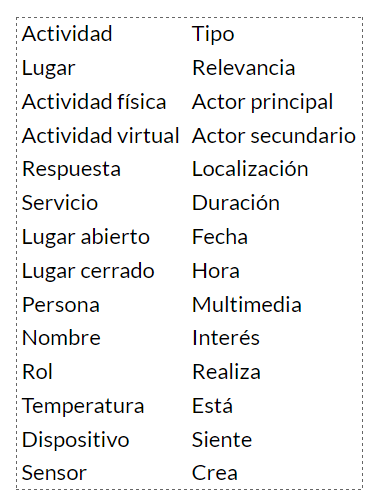
\includegraphics[width=0.3\textwidth]{Cap3/Images/Contexto_Modelado_Terminos}%
\caption{Terminos que relevantes de la ontología.} \label{fig:Contexto_Modelado_Terminos}
\end{figure}

Se realiza una lluvia de ideas teniendo en cuenta las acciones que desarrollan los usuarios de un sistema de contexto en diferentes casos de estudio luego algunas palabras son agrupadas y analizadas de acuerdo al conocimiento en el área. Las palabras resultantes se pueden observar en la figura \ref{fig:Contexto_Modelado_Terminos}


\textbf{\textit{(ii) considerar las ontologías que se pueden reutilizar}}

Luego de identificar los conceptos relevantes para la ontología se identifican los recursos usados en otras propuestas del estado del arte. Teniendo en cuenta que la búsqueda de ontologías en la actualidad no es tarea fácil dada la desactualización de las fuentes y los sistemas de búsqueda, se opta por el uso de fuentes encontradas en el sistema Linked Open Vocabularies (LOV) \footnote{http://lov.okfn.org/dataset/lov/} y propuestas por la W3C. A continuación se presenta la tabla \ref{tbl:Mod_Extern_Ontology} en donde se encuentran las ontologías usadas para ampliar los significados de las clases de la ontología de contexto.

\todo[]{https://www.w3.org/TR/activitystreams-vocabulary/}
Tener en cuenta y % https://www.w3.org/ns/activitystreams

% http://ld-r.org/



%IMPORT DE LA TABLA
\begin{table}[ht]
\centering
\caption{Recursos ontológicos externos}
\label{tbl:Mod_Extern_Ontology}
\begin{tabular}{lll}
\hline
\multicolumn{1}{c}{\textbf{Ontología de Contexto}}                                   & \multicolumn{1}{c}{\textbf{Ontología Externa}}                                              & \multicolumn{1}{c}{\textbf{Ejemplo de Componentes}} \\ \hline
\multicolumn{1}{l|}{Persona}                                                         & \multicolumn{1}{l|}{Foaf \tablefootnote{http://xmlns.com/foaf/spec/}}                                                                   & foaf:Agent, foaf:Person                             \\
% \multicolumn{1}{l|}{Rol}                                                             & \multicolumn{1}{l|}{Foaf \tablefootnote{http://xmlns.com/foaf/spec/}}                                                                   & foaf:Group                                          \\
\multicolumn{1}{l|}{\begin{tabular}[c]{@{}l@{}}Dispositivo\\  y Sensor\end{tabular}} & \multicolumn{1}{l|}{SSN \tablefootnote{https://www.w3.org/TR/vocab-ssn/}}                                                                    & sosa:Sensor, sosa:Observation                       \\
\multicolumn{1}{l|}{Multimedia}                                                      & \multicolumn{1}{l|}{\begin{tabular}[c]{@{}l@{}}OMR \tablefootnote{https://www.w3.org/ns/ma-ont}\\ M3 - adaptación\\ Dolce?\end{tabular}} & ma:MediaResource                                    \\
\multicolumn{1}{l|}{Lugar}                                                           & \multicolumn{1}{l|}{\begin{tabular}[c]{@{}l@{}}GeoNames \tablefootnote{http://www.geonames.org/ontology/documentation.html}\end{tabular}}              & geo:lat, geo:long, genames:nearby                   \\
\multicolumn{1}{l|}{Tiempo}                                                          & \multicolumn{1}{l|}{Time Ontology \tablefootnote{https://www.w3.org/TR/owl-time/}}                                                          & time:dayOfWeek, time:TemporalEntity                    \\ \hline
\end{tabular}
\end{table}


% \begin{table}[h!]
% \centering
% \caption{Recursos ontológicos externos}
% \label{tbl:Mod_Extern_Ontology}
% \begin{tabular}{lll}
% \hline
% \multicolumn{1}{c}{\textbf{Ontología de Contexto}}                                   & \multicolumn{1}{c}{\textbf{Ontología Externa}}                                              & \multicolumn{1}{c}{\textbf{Ejemplo de Componentes}} \\ \hline
% \multicolumn{1}{l|}{Persona}                                                         & \multicolumn{1}{l|}{Foaf \tablefootnote{http://xmlns.com/foaf/spec/}}                                                                   & foaf:Agent, foaf:Person                             \\
% \multicolumn{1}{l|}{\begin{tabular}[c]{@{}l@{}}Dispositivo\\  y Sensor\end{tabular}} & \multicolumn{1}{l|}{SSN \tablefootnote{https://www.w3.org/TR/vocab-ssn/}}                                                                    & sosa:Sensor, sosa:Observation                       \\
% \multicolumn{1}{l|}{Multimedia}                                                      & \multicolumn{1}{l|}{\begin{tabular}[c]{@{}l@{}}OMR \tablefootnote{https://www.w3.org/ns/ma-ont}\\ M3 - adaptación\\ Dolce?\end{tabular}} & ma:MediaResource                                    \\
% \multicolumn{1}{l|}{Lugar}                                                           & \multicolumn{1}{l|}{\begin{tabular}[c]{@{}l@{}}GeoNames \tablefootnote{http://www.geonames.org/ontology/documentation.html}\\ Schema \tablefootnote{http://schema.org/Place}\end{tabular}}              & geo:lat, geo:long, genames:nearby                   \\
% \multicolumn{1}{l|}{Tiempo}                                                          & \multicolumn{1}{l|}{Time Ontology \tablefootnote{https://www.w3.org/TR/owl-time/}}                                                          & time:dayOfWeek, time:hasDuration                    \\ \hline
% \end{tabular}
% \end{table}



% foaf = http://xmlns.com/foaf/spec/
% ssn =  https://www.w3.org/TR/vocab-ssn/
% time = https://www.w3.org/TR/owl-time/#time:dayOfWeek
% multimedia=  https://www.w3.org/ns/ma-ont
% location = http://www.geonames.org/ontology/documentation.html - http://schema.org/Place
\todo{Meter en la tabla Rol con foaf (no estoy seguro)}

% foaf = http://xmlns.com/foaf/spec/
% ssn =  https://www.w3.org/TR/vocab-ssn/
% time = https://www.w3.org/TR/owl-time/#time:dayOfWeek
% multimedia=  https://www.w3.org/ns/ma-ont
% location = http://www.geonames.org/ontology/documentation.html - http://schema.org/Place

\todo{Definir si la ontología con extensiones hace parte del dominio o de la upper}
\textit{\textbf{Esta ampliación hace parte de la ontología del dominio?}}\\


\textbf{\textit{(iv) definir la jerarquía de clases}}

Partiendo de los términos relevantes identificados en el paso (iii) de la metodología y siguiendo los indicios de las clases encontradas en el estado del arte se opta por modelar el contexto usando los siguientes conceptos \textbf{\textit{Persona, Rol, Actividad, Lugar, Sensor, Dispositivo, Servicio, Tiempo y Multimedia}}. Los términos que no se convierten en clases fueron analizados y seleccionados para convertirse en propiedades que describen o relacionan las entidades de la ontología.

\todo{Actualizar la jerarquía poniendo con objeto}
En la figura \ref{fig:Contexto_Modelado_Jerarquia} se presenta la jerarquía de la ontología de alto nivel. Dado que la ontología del dominio depende del caso de estudio esta se presenta con mayor detalle en la sección \ref{sec:CS_Ont_Dominio} en esta solo se mostrará la relación entre las nuevas clases incluidas.

\begin{figure}[!hb]
\centering%
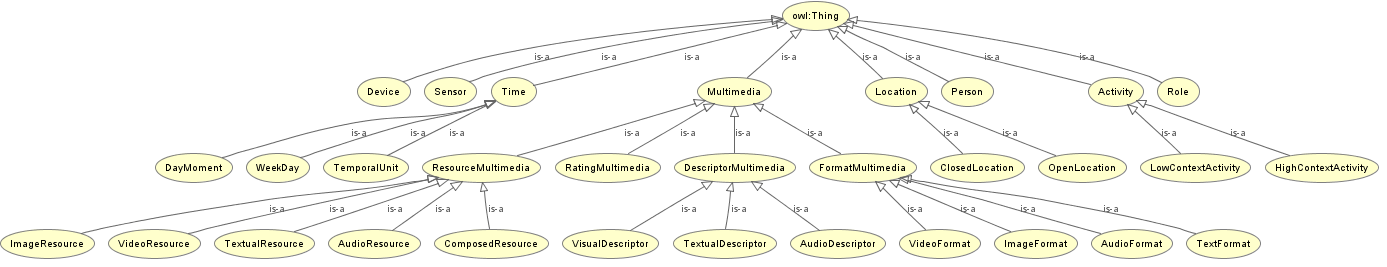
\includegraphics[width=\textwidth]{Cap3/Images/Contexto_Modelado_Jerarquia}%
\caption{Jerarquía de las clases de la ontología.} \label{fig:Contexto_Modelado_Jerarquia}
\end{figure}


\textbf{\textit{(v, vi) definir las propiedades de las clases y sus características}}

En esta etapa se identifican las propiedades de la ontología, se entienden propiedades como valores que describen entidades y relaciones existentes entre las entidades. En el diagrama \ref{fig:Contexto_Modelado_Relaciones} se puede ver la interacción entre las clases principales de la ontología por ejemplo un contenido multimedia describe una actividad y un dispositivo o una persona pueden crear contenidos multimedia.

\todo{Actualizar a nueva versión con objeto, poner versión de protégé?}
\begin{figure}[ht]
\centering%
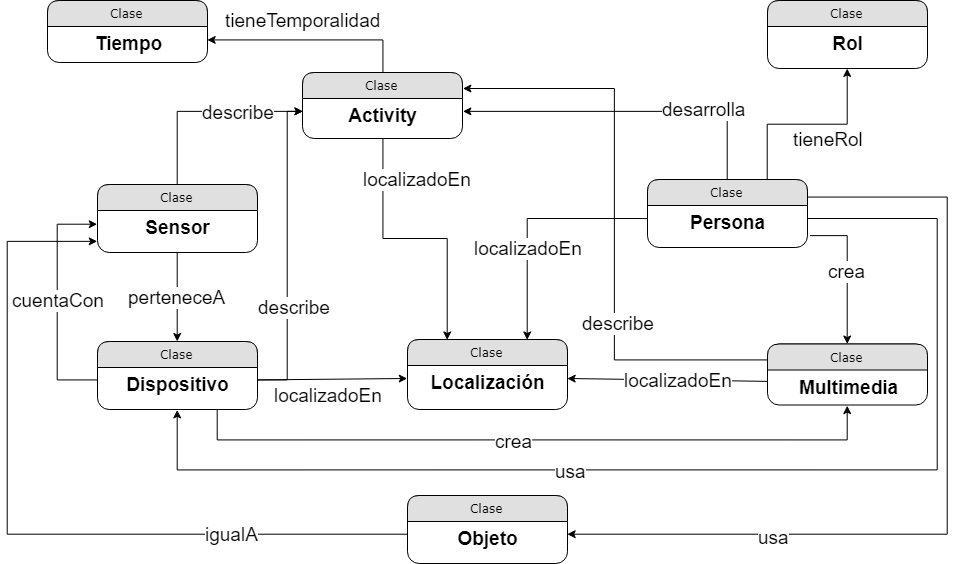
\includegraphics[width=0.8\textwidth]{Cap3/Images/Contexto_Modelado_Relaciones}%
\caption{Relaciones principales entre las clases de la ontología de contexto.} \label{fig:Contexto_Modelado_Relaciones}
\end{figure}

De otro lado en la figura \ref{fig:Contexto_Modelado_TipoDato} se presenta una pequeña parte de los valores que describen las clases y las características de estos valores. Por ejemplo la entidad persona tiene la propiedad nombre que es del tipo de dato Literal.

\begin{figure}[ht]
\centering%
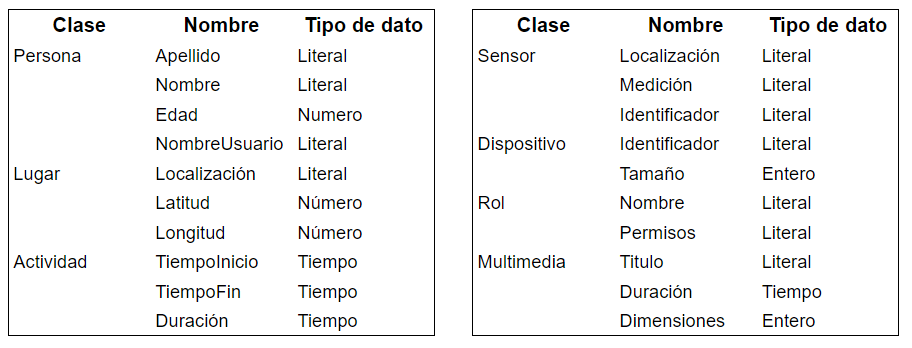
\includegraphics[width=0.9\textwidth]{Cap3/Images/Contexto_Modelado_Caract_Relaciones}%
\caption{Características de las propiedades de la ontología.} \label{fig:Contexto_Modelado_TipoDato}
\end{figure}



\textbf{\textit{(vii) poblar la ontología con los individuos necesarios}}

Esta etapa se desarrollará en la sección \ref{sec:CS_Ont_Dominio} cuando se desarrollen los componentes propios del dominio de la aplicación.


% En la figura \ref{Contexto_Upper_Ontology} se puede ver un extracto de la ontología de alto nivel con componentes de ontologías externas.


EN LA PÁGINA \textbf{http://www.visualdataweb.de/webvowl/#iri=http://purl.org/m-context/ontologies/mContext} SE PUEDE VER LA ONTOLOGÍA 